\section{Mehrdimensionale Differenzierbarkeit}
Für
\[
	f : \R \to \R  $ ist $ f^\prime (x_0) \coloneqq \lim_{\overset{x \to x_0}{x \neq x}} \frac{ f(x) - f(x_0) }{ x - x_0 }
\]
Umformuliert: $ f $ ist genau dann in $ x_0 \in \R  $ differenzierbar, wenn es eine lineare Abbildung $ L : \R \to \R  $ so, dass
\[
	\lim_{\overset{h \to 0}{h \neq 0}} \frac{ \left| f (x_0 + h) - f(x_0) - L(h) \right| }{ \left| h \right|  } = 0
\]
mit $ L(h) = f^\prime (x_0) \cdot h $, $  h $ ein Vektor

\begin{definition}[Differenzierbarkeit]
	Sei $ \Omega \subset \R ^n $ offen und $ x_0 \in \Omega $.
	Wir nennen $ f: \Omega \to \R $ \textbf{differenzierbar in $ x_0 $}, falls eine lineare Abbildung $ L : \R ^n \to \R  $ existiert mit
	\[
		\lim_{\overset{h \to 0}{h \neq 0}} \frac{ \left| f(x_0 + h) - f(x_0) - L(h) \right| }{ \left| h \right|  } = 0.
	\]
	($ h $ Vektor)\\
	Wir nennen $ D f(x_0) \coloneqq L $ die \textbf{totale Ableitung} von $ f $ in $ x_0 $

	Umformuliert: Mit $ R(x_0, h) \coloneqq \left| f(x_0 + h) - f(x_0) - L(h) \right|  $, ist die Differenzierbarkeit von $ f $ in $ x_0 $ äquivalent zu
	\[
		\lim_{\overset{h \to 0}{h \neq 0}} \frac{ R(x_0, h) }{ \left| h \right|  } = 0.
	\]
	Daraus folgt die Eindeutigkeit der totalen Ableitung.
	Ist $ \tilde L $ eine weitere, so folgt für jeden Einheitsvektor
	\[
		e_i = ( 0, \dotsc, 0, \underbrace{1}_{i\text{-te Stelle} }, 0, \dotsc, 0)
	\]
	\[
		(L - \tilde L) (e_i) = \lim_{t \searrow 0} \frac{( L - \tilde L )(t e_i) }{ \left| t e_i \right|  } = 0 \implies L = \tilde L
	\]
	Ist $ h = (h_1, \dotsc, h_n)^T \in \R ^n $, so schreibe 
	\[
		h = \sum_{i=1}^{n} h_i e_i
	\]
	Damit folgt
	\[
		D f(x_0) (a) = L(h) = \sum_{i=1}^{n} L(h_i e_i) = \sum_{i=1}^{n} h_i L(e_i)
	\]
	Deswegen definieren wir
	\[
		\nabla f(x_0) \coloneqq \left( L(e_1) , \dotsc, L(e_n) \right) 
	\]
	Damit gilt der Zusammenhang $ D f(x_0) (h) = \nabla f(x_0) \cdot h $
\end{definition}

\begin{example}
	Sei $ f(x) = Ax + b $ mit $ A \in \R ^{1 \times n}  $ und $ b \in \R  $.
	Dann ist $ L(h) \coloneqq Ah $ und $ \nabla f(x_0) = A $ f.a. $ x_0 \in \R ^n $.
\end{example}
\begin{example*}
	Sei $ A = (a_{ij})_{1 \leq i, j \leq n} \in \R ^{n \times n}  $ eine symmetrische Matrix (d.h. $ a_{ij} = a_{ji}  $).
	Wir betrachten $ f(x) \coloneqq x^t (Ax) \left( = \left<x, Ax \right> \right)  $.
	Für $ x_0 \in \R ^n $ gilt $ f(x_0 + h) - f(x_0) = 2x_0^t Ah + h^t Ah $.
	Definiere $ L(h) \coloneqq 2x_0^tAh $.
	Dann ist $ L $ eine lineare Abbildung von $ \R ^n $ nach $ \R  $ und für $ R(h) \coloneqq h^tAh $ gilt, dass $ \left| R(h) \right| \leq c \left| h \right| ^2 $.
	Also $ \nabla f(x_0) = 2x_0^t A $
\end{example*}
\textbf{Anschauliche Interpretation}
\[ \Graph(f) \coloneqq \left\{ (x, f(x)) : x \in \Omega \right\} \subset \R ^{n + 1}  \text{(Graph von $ f $)}. \]
Ist $ f  $ in $ x_0 $ differenzierbar, so gibt uns
\[
	T_{f_{x_0} } \coloneqq f(x_0) + \nabla f(x_0) (x - x_0)
\]
eine affin-lineare Approximation von $ f $ in $ x_0 $ .\\
Der Graph von $ T_{f_{x_0} }  $ 
also $ \Graph(T(f_{x_0} ) \coloneqq \left\{ (x, x_{n + 1} ) : x_{n + 1} = T_{f_{x_0}} (x) \right\}  $ heißt \textbf{Tangentialhyperebene}

\setcounter{environmentnumber}{3}
\begin{theorem}
	Sei $ \Omega \subset \R ^n $ und $ f : \Omega \to \R  $ differenzierbar in $ x_0 $.
	Dann ist $ f  $ stetig in $ x_0 $.
\end{theorem}
\begin{subproof*}[Theorem \ref{4.4}]
	Folgt direkt aus der Differenzierbarkeit, denn
	\[
		\left| f(x_0) - f(x_0) \right| \leq \left| \nabla f(x_0) \cdot h + R(h) \right| \overset{\left| h \right| \to 0}{\longrightarrow} 0
	\]
\end{subproof*}

\subsection{Partielle Ableitung}
\begin{subdefinition*}[Niveaumenge]
	Sei $ f: U \to \R  $ $ \left( U \subseteq \R ^n \right)  $, dann definiere die Niveaumengen für $ c \in \R : $ 
	\[
		N_f (c) \coloneqq \left\{ x \in U : f(x) = c \right\} \subset \R ^n
	\]
\end{subdefinition*}

\begin{definition}[Partielle Ableitungen]
	Sei $ U \subseteq \R ^n $ offen und $ f: U \to  \R  $.
	Dann heißt $ f $ im Punkt $ x_0 \in U $ \textbf{partiell differenzierbar in der $ i $-ten Koordinate}, falls der Limes
	\[
		D_i f(x) \coloneqq \lim_{\underset{h \neq  0}{h \to  0}} \frac{ f(x + e_i h) - f(x) }{ h } 
	\]
	existiert und endlich ist mit $ e_i \coloneqq (0, \dotsc, 0, \underbrace{1}_{i\text{-te} }, 0 , \dotsc, 0) $.
	Sei $ x = (x_1, \dotsc, x_n) \in U $.
	Für $ i = 1, \dotsc, n $ betrachte die Funktion
	\[
		\xi \mapsto f_i(\xi) \coloneqq f( x_1, \dotsc, x_{i - 1} , \xi, x_{i + 1} , \dotsc, x_n).
	\]
	Dann folgt direkt aus Definition \ref{4.5}, dass
	\[
		D_i f(x) = \lim_{h \to 0} \frac{ f_i(x_i + h) - f_i(x_i) }{ h } = f_i^\prime (x_i). 
	\]
	
\end{definition}

\begin{definition}[(stetige) partielle Differenzierbarkeit]
	Sei $ U \subseteq \R ^n $ offen.
	Dann heißt eine Funktion $ f : U \to \R  $ \textbf{partiell differenzierbar}, falls $ D_i f(x) $ f.a. $ x \in U $ und alle $ i = 1, \dotsc, n $ existiert.
	$ f $ heißt stetig partiell differenzierbar, falls zusätzlich alle partiellen Ableitungen $ D_i f_i U \to \R  $ stetig sind.\\
	\textbf{Schreibweise:} statt $ D_i f $ schreibt man auch
	\[
		\frac{\partial f}{ \partial x_i } 
	\]
	Entsprechend
	\[
		D_i f(x) = \frac{ \partial f }{ \partial x_i } (x) = \frac{ \partial f(x) }{ \partial x_i } .
	\]
\end{definition}

\begin{example}
	\[
		F : \R ^2 \to \R , (x, y) \mapsto F(x, y) \coloneqq \exp (x^2 + y^2)
	\]
	Für $ f(x) \coloneqq \exp (x^2 + c^2) $ gilt $ f^\prime (x) = 2x \exp (x^2 + c^2) $. D.h.
	\[
		\frac{\partial}{ \partial x } F(x, y) = \frac{ \partial }{ \partial x } \exp (x^2 + y^2) = 2x \exp (x^2 + y^2)
	\]
	und analog
	\[
		\frac{ \partial }{ \partial y } F(x, y) = 2y \exp (x^2 + y^2).
	\]
\end{example}

\begin{example}
	Betrachte $ r : \R ^n \to \R  $, $ r(x) \coloneqq  \left\| x \right\| _2 = \sqrt{x_1^2 + x_2^2 + \dotsb + x_n^2}  $.
	Die Niveaumengen
	\[
		N_f(c) = \left\{ x \in \R ^n : r(x) = c \right\} 
	\]
	sind Sphären mit Radius $ c > 0 $.\\
	\begin{tikzpicture}
		\begin{axis}[
			xmin= -1, xmax= 1,
			ymin= -1, ymax = 1,
			axis lines = middle,
			xtick = {2 * floor(-1/2) + 1, 1},
			ytick = {-1, 1},
			height = 4cm,
			width = 4cm,
		]
			\addplot[parametric, domain=-4:4, samples=100] function{cos(t), sin(t)};
			\addplot[parametric, domain=-4:4, samples=100] function{0.667 * cos(t), 0.667 * sin(t)};
			\addplot[parametric, domain=-4:4, samples=100] function{0.333 * cos(t), 0.333 * sin(t)};
		\end{axis}
	\end{tikzpicture}\\
	\textbf{Beh.:} Die Funktion $ r $ ist in $ \R ^n \setminus \left\{ 0 \right\}  $ partiell differenzierbar und es gilt
	\[
		\frac{\partial r}{ \partial x_i } (x) = \frac{x_i}{ r_i } 
	\]
	für $ x \neq 0 $.\\
	Für $ x \neq 0 $ 
	\[
		\frac{ \dd }{ \dd x } \left| x \right| = \frac{ x }{ \left| x \right|  } = \begin{cases}
			-1 & \quad \text{für $ x < 0 $} \\
			1 & \quad \text{für $ x > 0 $} 
		\end{cases}
	\]
	``Beweis'' der Behauptung:\\
	Betrachte $ \xi \mapsto \sqrt{x_1^2 + \dotsb + \xi^2 + \dotsb + x_n^2}  $, das ist differenzierbar! 
	Es gilt
	\[
		\frac{ \partial r }{ \partial x_i } = \frac{ \partial }{ \partial x_i } (x_1^2 + \dotsb + x_i^2 + \dotsb + x_n^2)^{\frac{ 1 }{ 2 } } = 2x_i \cdot \frac{ 1 }{ 2 } \left( x_1^2 + \dotsb + x_i^2 + \dotsb + x_n^2 \right) ^{-\frac{ 1 }{ 2 } } = - \frac{x_i}{ r(x) } 
	\]
\end{example}

\begin{example}
	Sei $ n \geq 2 $ betrachte $ F(x) : \begin{cases}
		\frac{ x_1 \cdot x_2 \dotsb x_n }{ r(x)^n } & \quad \text{für $ x \neq 0 $} \\
		0 & \quad \text{für $ x = 0 $} 
	\end{cases} $ 
	In $ \R ^n \setminus \left\{ 0 \right\}  $ ist $ F $ partiell differenzierbar (nach vorherigem Beispiel).
	Für die partielle Ableitung nach $ x_1 $ gilt
	\[
		\frac{\partial F(x)}{ \partial x_1 } = \frac{ x_2 \dotsb x_n }{ r_n } - n \frac{ x_1^2 x_2 \dotsb x_n }{ r^{n + 2}  } .
	\]
	Analog für partielle Ableitung in Richtung $ x_i $
	$ F $ ist auch in $ x = 0 $ partiell differenzierbar mit
	\[
		\frac{ \partial F}{ \partial x_i } (0) = \lim_{h \to 0} \frac{ F(h \cdot e_i ) - F(0) }{ h } = 0.
	\]
	$ \implies F $ ist auf ganz $ \R ^n $ partiell differenzierbar.\\
	\textsc{Aber:} $ F $ ist in $ x_0 = 0 $ nicht stetig, denn betrachte $ a_k = \left( \frac{ 1 }{ k } , \dotsc, \frac{ 1 }{ k }  \right) , k \geq 1 $.
	Es gilt $ r (a_k) = \frac{ \sqrt{n} }{ k }  $, also $ F(a_k) = \frac{ \left( \frac{ 1 }{ k }  \right) ^n }{ \left( \frac{\sqrt{n}}{ k }  \right) ^n } = n^{- \frac{n}{ 2 } } \neq 0 = F(0) $.\\
	{\color{gadse-red}Also: Partiell differenzierbar $ \nRightarrow  $ stetig.}
\end{example}

\textbf{Beobachtung:} Komponenten von $ \nabla f(x) $ sehen aus wie
\[
	\lim_{\left| h \right|  \to 0} \frac{ \left| f(x + h e_i ) - f(x) \right| }{ \left| h \right|  } .
\]
D.h. $ \nabla f(x) = \left( \frac{ \partial f }{ \partial x_1 } (x) , \dotsc, \frac{\partial f}{ \partial x_n } (x) \right)  $ und (totale) Differenzierbarkeit $ \implies  $ partielle Differenzierbarkeit.

\begin{example}
	$ \nabla r(x) = \frac{ x }{ r }  $ und $ \nabla f(r) = f^\prime (r) \frac{ x }{ r }  $, zum Beispiel $ \nabla  \frac{ 1 }{ r } = - \frac{ x }{ r^3 }  $ 
	(Manche schreiben ``$ \grad $'' statt ``$ \nabla  $'')
\end{example}

\begin{example}
	Seien $ f, g : U \to \R  $ zwei partiell differenzierbare Funktionen. Dann
	\[
		\nabla (fg) = g \cdot \nabla f + f \cdot \nabla g.
	\]
\end{example}

\begin{definition}[Divergenz]
	Sei $ \Omega \subset \R ^n $ und $ v = v_1, \dotsc, v_n) : \Omega \to \R ^n $ ein partiell differenzierbares Vektorfeld (VF = Abbildung nach $ \R ^n $, partiell differenzierbar = jede Komponente ist partiell differenzierbar).
	Dann definiere Divergenz von $ V $ durch
	\[
		\Div v \coloneqq \sum_{k=1}^{n} \frac{ \partial }{ \partial x_k } v_k
	\]
	\textbf{Bemerkung:} Formal kann man schreiben
	\[
		\Div v = \left< \nabla , v \right> = \sum_{i=1}^{n} \frac{ \partial }{ \partial x_i } v_i.
	\]
	\textbf{Rechenregel:}
	\[
		\frac{ \partial }{ \partial x_i } (f v_i) = \frac{\partial f }{ \partial x_i } v_i + f \frac{ \partial v_i }{ \partial x_i } \quad (f : U \to \R ^n ).
	\]
	$ \implies \Div (f v) = \left< \nabla f, v \right> + f \cdot \Div v $.
	(Formal $ \left< \nabla , fv \right> = \left<\nabla  f, v \right> + f \left<\nabla , v \right> $.
\end{definition}

\begin{example*}
	$ F : \R ^n \setminus \left\{ 0 \right\} \to \R ^n, F(x) \coloneqq \frac{ x }{ r(x) }  $.\\
	Da
	\[
		\Div x = \sum_{i=1}^{n} \frac{ \partial x_i }{ \partial x_i } = n \text{ und} 
	\]
	\[
		\left<x, x \right> = r^2(x).
	\]
	Damit folgt
	\[
		\Div \frac{ x }{ r } = \left< \nabla \frac{ 1 }{ r } , x \right> + \frac{ 1 }{ r } \Div x = \left< - \frac{ x }{ r^3 } , x \right> + \frac{ n }{ r }  = \frac{ n - 1 }{ r } 
	\]
\end{example*}

\subsection{Höhere Ableitungen und Satz von Schwarz}
\begin{theorem}[Schwarz]
	Sei $ \Omega \subset \R ^n $ und $ u : \Omega \to \R  $ zweimal stetig partiell differenzierbar in $ \Omega $.
	Dann gilt f. a. $ 1 \leq i, j \leq n $, dass
	\[
		\frac{ \partial }{ x_i } \cdot \frac{ \partial }{ x_j } u = \frac{ \partial }{ x_j } \cdot \frac{ \partial }{ x_i } u.
	\]
	
\end{theorem}

\textbf{$ \R  $ versus $ \R ^n $:}\\
Im $ \R  $ gibt es zwei Möglichkeiten.\\
Im $ \R ^n $ gibt es unendlich viele Möglichkeiten.

Zwei (drei) Möglichkeiten, über Differenzierbarkeit zu sprechen:
\begin{itemize}
	\item Zurückführen auf die 1-dim Situation.
		\[
			x_j \mapsto f( \underbrace{ x_1, \dotsc, x_{j - 1} }_{\text{friere ein} } , x_{j} , \underbrace{ x_{j + 1} , \dotsc, x_n }_{\text{friere ein} } )
		\]
		``$ j $-te partielle Funktion''
		\[
			\partial_j f(x_0) \coloneqq \lim_{\underset{h \neq 0}{h \to 0} } \frac{ f_j (x_j + h) - f_j(x_j) }{ h } 
		\]
		($ h $ ist eine Zahl, also $ h \in \R  $)
	\item \textbf{Richtungsableitungen}: $ \nu \in \mathdollar^{n - 1} = \left\{ x \in \R ^n : \left| x \right|  = 1 \right\}  $ (mit $ \left| \cdot  \right|  $ Euklidische Norm $ \left| x \right| \coloneqq \left\| x \right\| _2 $)
		\[
			\partial_{\nu} f(x_0) \coloneqq \lim_{\underset{h \neq 0}{h \to 0}} \frac{ f(x_0 + h \nu) - f(x_0) }{ h } 
		\]
		($ h $ ist eine Zahl, also $ h \in \R  $)
		Hierbei interessiert nur, was $ f $ entlang $ x_0 + \R \nu $ macht.
		Dies liefert \textbf{eine} Art der Ableitung:\\
		Richtungsableitung entlang $ \nu $.
		Partielle Ableitung entspricht Richtungsableitung bezüglich $ \nu \in \left\{ e_1, \dotsc, e_n \right\}  $.
		Jede Richtung $ \nu $ lässt sich als $ \nu = \sum_{i=1}^{n} \lambda_i e_i $ schreiben - können wir also Richtungsableitungen über partielle Ableitungen ausdrücken? $ \to  $ Ja, später.
	\item Linearisierbarkeit: In 1-dim Differenzierbarkeit entspricht lokale Approximierbarkeit durch affin-lineare Funktion entspricht Approximierung des Graphen durch Tangenten\\
		$ \rightsquigarrow $ Differenzierbarkeit entspricht Approximierbarkeit (lokal) durch affin-lineare Funktionen (!) entspricht Approximierbarkeit des Graphen durch affine Hyperebenen.
\end{itemize}

\begin{subdefinition*}[Hyperebenen]
	Hyperebene $ (n - 1) $-dim. Untervektorräume im $ \R ^n $.\\
	Algebraische Charakterisierung:
	\[
		\Phi \in (\R ^n)^*. \quad \Kern\left( \Phi \right) .
	\]
\end{subdefinition*}
\begin{subdefinition*}[Affin-lineare Hyperebenen]
	\[
		x_0 + \Kern\left( \Phi \right) = \left\{ x_0 + y : \Phi(y) = 0 \right\} 
	\]
	\begin{itemize}
	{\color{gadse-orange}
		\item $ \Phi(x_1, x_2, x_3) \coloneqq x_1 $, $ \Kern\left( \Phi \right) = \left\{ \begin{pmatrix} 0 \\ y \\ z \end{pmatrix} : y, z \in \R  \right\} $\\
				$ x_0 + \Kern\left( \Phi \right)  $, Ebene parallel zur $ x_2, x_3 $-Ebene
	}
		\item $ \mathbb{E} = \left\{ (x_1, x_2, x_3) : 3x_1 + 2x_2 - x_3 = 1 \right\} = x_0 + \Kern(\Phi) $ 
		\item $ f(x_1, x_2) = e^{-x_1^2 - x_2^2}, x \mapsto e^{-x^2}   $
	\end{itemize}
\end{subdefinition*}

\textbf{Ziel:} Differenzierbarkeit $ \implies  $ partielle Differenzierbarkeit ($ \impliedby  $ falls partielle Ableitung stetig)

\setcounter{environmentnumber}{14}
\begin{theorem}[Schwarz]
	Sei $ \Omega \subset \R ^n $ offen und $ f : \Omega \to \R  $ zwei mal stetig partiell differenzierbar (d.h., die zweite partiellen Ableitungen $ \partial_i \partial_j f $ existieren und sind stetig) in $ x_0 \in \Omega $, so gilt:
	\[
		\partial_i \partial_j f(x_0) = \partial_j \partial_i f(x_0)
	\]
\end{theorem}

\textbf{MWS:} $ g : \R \supset I \to \R   $ differenzierbar, $ -\infty < a < b < \infty $, so $ \exists \xi \in [a, b] $:
\[
	g^\prime \left( \xi \right) = \frac{ g(b) - g(a) }{ b - a } 
\]

\begin{proof*}[Theorem \ref{4.15}]
	\OE{} $ n = 2 $. $ i = 1, j = 2 $.
	$ (x_1, x_2)  $ entspricht $ (x, y) $.\\
	$ \Omega $ offen $ \implies \exists \delta > 0 : \left\{ (x, y) : \left| x \right| < \delta, \left| y \right| < \delta \right\} \subset \Omega $, wobei \OE{} $ x_0 = 0 $
	\begin{enumerate}[label=(\arabic*)]
		\item Fixiere $ y \in \R  $ mit $ \left| y \right| < \delta $. Definiere
			\[
				F_y : (- \delta, \delta) \ni x \mapsto f(x, y) - f(x, 0) \in \R 
			\]
			Mit \textbf{MWS}
			\begin{equation}
				\label{eq:4.15.1}
				\tag{$\heartsuit$}
				\exists \xi \in \R : \left| \xi \right| \leq \left| x \right| : F_y^\prime (\xi) x = F_y - F_y(0)
			\end{equation}
			\[
				F_y^\prime (\xi) = (\partial_1 f) (\xi, y) - (\partial_1 f)(\xi, 0).
			\]
			\textbf{Wiederum} MWS.
			\begin{equation}
				\label{eq:4.15.2}
				\tag{$\heartsuit\heartsuit$}
				\exists \eta \in \R : \left| \eta \right| \leq \left| y \right| : (\partial_1 f)(\xi, y) - (\partial_1 f)(\xi, 0) = \partial_2\partial_1 f(\xi, \eta) \cdot y
			\end{equation}
			\textbf{Hiermit:}
			\begin{align*}
				~&f(x, y) - f(x, 0) - f(0, y) + f(0, 0) \\
				=& \underbrace{( f(x, y) - f(x, 0) )}_{=F_y(x)} - \underbrace{( f(0, y) - f(0, 0)}_{ = F_y(0)} \\
				\overset{\text{Def.} }{=} & F_y (x) - F_y(0) \\
				\overset{\eqref{eq:4.15.1}}{=} F_y^\prime (\xi) \cdot x\\
				\label{eq:4.15.3}
				\tag{\dag}
				\overset{\eqref{eq:4.15.2}}{=} \partial_2 \partial_1 f(\xi, \eta) x \cdot y
			\end{align*}
		\item Fixiere nun $ x $, betrachte $ G_x(y) \coloneqq  f(x, y) - f(0, y) $. Analog wie für (1):
			\[
				\exists \tilde \eta \in \R : \left| \tilde \eta \right| \leq  \left| y \right| : G_x (y) - G_x(0) = G_x^\prime (\tilde \eta) \cdot y.
			\]
			Daneben mit MWS
			\[
				\exists \tilde \xi \in \R : \left| \tilde \xi \right| \leq \left| x \right| : G_x^\prime (\tilde \eta) = \partial_2 f(x, \tilde \eta) - \partial_2 f(0, \tilde \eta) = \partial_1 \partial_2 f(\tilde \xi, \tilde \eta) \cdot x
			\]
			$ \implies f(x, y) - f(x, 0) - f(0, y) + f(0, 0) = \partial_1 \partial_2 f(\tilde \xi, \tilde \eta) xy $\\
			$ \overset{\eqref{eq:4.15.3}}{\implies } \partial_2 \partial_1 f(\xi, \eta) xy = \partial_1 \partial_2 f(\tilde \xi, \tilde \eta) xy $\\
			$ \overset{xy \neq 0}{\implies } \partial_2 \partial_1 f(\xi, \eta) = \partial_1\partial_2 f(\tilde \xi, \tilde \eta) $
			hier hängen aber $ \xi, \tilde \xi $ von $ x $ und $ \eta, \tilde \eta $ von $ y $ ab.
			Nach Konstruktion:
			$ (x, y) \to (0, 0) \implies (\xi, \eta), (\tilde \xi, \tilde \eta) \to 0 $.
			Da $ f $ \textbf{zweimal stetig partiell differenzierbar:}
			\[
				\partial_1 \partial_2 f(0, 0) = \lim_{(\tilde \xi, \tilde \eta) \to (0, 0)} \partial_1 \partial_2 f(\tilde \xi, \tilde \eta) = \lim_{(\xi, \eta) \to (0, 0)}  \partial_2 \partial_1 f(\xi, \eta) = \partial_2 \partial_1 f(0, 0).\qed
			\]
			Dies kann iteriert werden:
			$ f : \Omega \to \R  $ $ k $-mal stetig partiell differenzierbar und $ \pi  : \left\{ 1, \dotsc, k \right\} \to \left\{ 1, \dotsc, k \right\}  $ Permutation (d.h. bijektiv), so gilt für alle $ i_1, \dotsc, i_k \in \left\{ 1, \dotsc, n \right\} : $ 
			\[
				\partial_{i_1} \dotsb \partial_{i_k} = \partial_{i_{\pi (1)} } \dotsb \partial_{i_{\pi (k)} } f.
			\]
			
	\end{enumerate}
\end{proof*}

\textbf{Satz von Schwarz:} $ \Omega \subset \R ^n $ offen, $ f: \Omega \to \R  $ zwei mal stetig partiell differenzierbar $ \implies \forall i, j \in \left\{ 1, \dotsc, n \right\} : \partial_i \partial_j f = \partial_j \partial_i f. $
\[
	\frac{ \partial }{ \partial x_i } f \coloneqq \partial_i f.
\]
\begin{itemize}
	\item Damit: $ Hf = \nabla ^2 f \coloneqq \left( \partial_{ij} f \right) _{i, j \in \left\{ 1, \dotsc, n \right\} }  $ (\textbf{Hessematrix}).
		Mit Schwarz ist dies eine \textbf{symmetrische Matrix} (Bei Fr. Kuhlmann besonders aufpassen).
		\[
			A = A^{T} .
		\]
		Dann gibt es eine Basis $ v_1, \dotsc, v_n \in \R ^n $: Darstellende Matrix
		\[
			\begin{pmatrix} \lambda_1 & & 0\\ & \ddots & \\0 & & \lambda_n \end{pmatrix} .
		\]
		Dann z.B. $ v_1 $ entspricht $ \begin{pmatrix} 1 \\ 0 \\ \vdots \\ 0 \end{pmatrix}  $, also
		\[
			\begin{pmatrix} \lambda_1 & & 0\\ & \ddots & \\0 & & \lambda_n \end{pmatrix} \begin{pmatrix} 1 \\ 0 \\ \vdots \\ 0 \end{pmatrix} = \begin{pmatrix} \lambda_1 \\ 0 \\ \vdots \\ 0 \end{pmatrix} 
		\]
		$ \implies  $ Abbildung verhält sich auf $ \Span \left\{ v_1 \right\}  $ wie Streckung.
\end{itemize}

\begin{example}[Rotation und Gradient]
	$ f : \R \to \R  $ 
	\[
		\nabla f = \begin{pmatrix} \partial_1 f \\ \vdots \\ \partial_n f \end{pmatrix} .
	\]
	Falls $ n = 3 $ definiere \textbf{Rotation} (``curl'') von $ v = \begin{pmatrix} v_1 \\ v_2 \\ v_3 \end{pmatrix} : \R ^3 \to \R ^3 $ durch
	\[
		\Rot(v) = \begin{pmatrix} \partial_1 \\ \partial_2 \\ \partial_3 \end{pmatrix} \times \begin{pmatrix} v_1 \\ v_2 \\ v_3 \end{pmatrix} 
		\coloneqq  \begin{pmatrix}
			\partial_2 v_3 - \partial_3 v_2 \\
			\partial_3 v_1 - \partial_1 v_3 \\
			\partial_1 v_2 - \partial_2 v_1 \\
		\end{pmatrix} 
	\]
	Die Rotation annihiliert den Gradienten \fbox{$ \Rot\left( \nabla f \right) = 0 $} $ \forall f : \R ^3 \to \R  $ zweimal stetig partiell differenzierbar (beachte: $ \nabla f : \R ^3 \to \R ^3 $)
	\[
		\Rot\left( \nabla f \right) =
		\begin{pmatrix} 
			\partial_1 \\
			\partial_2 \\
			\partial_3 \\
		\end{pmatrix} 
		\times 
		\begin{pmatrix} 
			\partial_1 f \\
			\partial_2 f \\
			\partial_3 f \\
		\end{pmatrix} 
		=
		\begin{pmatrix} 
			\partial_2 \partial_3 - \partial_3 \partial_2 f \\
			\partial_3 \partial_1 - \partial_1 \partial_3 f \\
			\partial_1 \partial_2 - \partial_2 \partial_1 f \\
		\end{pmatrix} 
		\overset{\text{Schwarz} }{=}
		\begin{pmatrix} 
			0 \\ 0 \\ 0
		\end{pmatrix} 
	\]
\end{example}

\begin{lemma*}[Poincar\'e-Lemma]
	\textbf{Für später} Ist $ \Rot(v) = 0 $, gibt es ein $ f : \R ^3 \to \R : v = \nabla f ? $ (Ja, aber nur in $ \R ^3 $, nicht in $ \Omega $)
\end{lemma*}

\begin{example}
	Die \textbf{Divergenz} von $ f: \R ^n \supset \Omega \to \R ^n $ ist definiert als
	\[
		\Div (f) = \sum_{i=1}^{n} \partial_i f_i.
	\]
	\[
		f = \begin{pmatrix} f_1 \\ \vdots \\ f_n \end{pmatrix} .
	\]
	\textbf{Beh.:} \fbox{$ \Div ( \Rot (g) ) = 0 $} Mit \textbf{Schwarz:}
	\[
		g =
		\begin{pmatrix} 
			g_1 \\ g_2 \\ g_3
		\end{pmatrix}
	\]
	\begin{align*}
		\Div
		\begin{pmatrix} 
			\partial_2 g_3 - \partial_3 g_2 \\
			\partial_3 g_1 - \partial_1 g_3 \\
			\partial_1 g_2 - \partial_2 g_1 \\
		\end{pmatrix} 
		  &= \partial_1 \left( \partial_2 g_3 - \partial_3 g_2 \right) 
		  + \partial_2 \left( \partial_3 g_1 - \partial_1 g_3 \right) 
		  + \partial_3 \left( \partial_1 g_2 - \partial_2 g_1 \right) \\
		  &\overset{\text{Schwarz} }{=} 0
	\end{align*}
	Damit: Divergenz annihiliert Rotation.
	\[
		f \to \nabla f \to \Rot( \nabla f ) \equiv 0
	\]
	\[
		g \to \Rot g \to \Div( \Rot g ) = 0
	\]
	\[
		\R \overset{\nabla }{\longrightarrow} \R ^3 \overset{\Rot}{\longrightarrow} \R ^3 \overset{\Div}{\longrightarrow} \R 
	\]
	``\textbf{Differentialkomplex}''
\end{example}

\begin{example}
	Für $ \Omega \subset \R ^n $ offen und $ f : \Omega \to \R ^n $ zweimal stetig partiell differenzierbar:
	\[
		\Delta f = \sum_{i=1}^{n} \partial_i \partial_i f \left( \eqcolon \sum_{i=1}^{n} \partial_i^2 f \right) 
	\]
	``Laplace-Operator''\\
	Das ist die Spur ($ \hat{=}  $ Summe über Diagonal  Diagonalelemente) der Hessematrix.
	Ist $ f : \Omega \to \R ^n $ zweimal stetig partiell differenzierbar mit \fbox{$ \Delta f = 0 $}, so heißt $ f $ \textbf{harmonisch}.
	(Erstes Beispiel einer partiellen Differentialgleichung)
	
\end{example}

\begin{itemize}
	\item $ f(x) = a \cdot x + b, a \in \R ^n, b \in \R $, $ \Delta f = 0 $.
	\item $ f(x) = \varphi\left( \left| x \right|  \right)  $, mit $ \varphi: [0, \infty) \to [0, \infty), \left| x \right| \coloneqq \left\| x \right\| _2 $
\end{itemize}

\textbf{Frage:} Wie muss $ \varphi $ aussehen?
\[
	f(x) = \varphi( \left| x \right| ).
\]
Dann $ \partial_i f(x) = \varphi^\prime (\left| x \right| ) \frac{ x_i }{ \left| x \right|  }  $
\[
	\partial_i \partial_i f(x) = \partial_i \left( \varphi^\prime \left( \left| x \right|  \right) \frac{ x_i }{ \left| x \right|  }  \right) = \varphi^{\prime \prime} \left( \left| x \right|  \right) \frac{ x_i^2 }{ \left| x \right| ^2 } + \varphi^\prime \left( \left| x \right|  \right) \frac{ \left| x \right| - x_i \frac{x_i }{ \left| x \right|  } }{ \left| x \right| ^2 } = \varphi^{\prime\prime} \left( \left| x \right|  \right) + \varphi^\prime \left( \left| x \right|  \right) \frac{ \left| x \right| ^2 - x_i^2 }{ \left| x \right| ^3 } ,
\]
also
\[
	0 \overset{!}{=} \Delta f \overset{\text{Def} }{=} \sum_{i=1}^{n} \partial_i \partial_i f = \varphi^{\prime\prime} \left( \left| x \right|  \right) + \varphi^{\prime} \left( \left| x \right|  \right) \frac{ n }{ \left| x \right|  } - \varphi^\prime \left( \left| x \right|  \right) \frac{ 1 }{ \left| x \right|  } .
\]
Setze \fbox{$ r \coloneqq \left| x \right|  $}
\begin{align*}
	&\implies 0 = \varphi^{\prime\prime} (r) + \frac{\varphi^\prime (r) }{ r } (n - 1) \\
	&\implies \frac{1 - n }{ r } \psi(r) = \psi^\prime (r), \text{ wobei \fbox{$ \psi \coloneqq \varphi^\prime  $}} \\
	&\overset{\text{\OE{} $ \psi \neq 0 $} }{\implies } \frac{1 - n}{ r } =  \fbox{$ \frac{ \psi^\prime (r) }{ \psi (r) }  $} = (\log (\psi(r)))^\prime .\\
	&\implies \int_{1}^{r} \frac{ 1 - n }{ s } \dd s = \int_{1}^{r} ( \log ( \psi (s ) ) )^\prime  \dd s = \log (\psi(r)) + C \\
	&\implies (1 - n) \log (r) = \log (\psi(r)) + C {\color{gadse-red} \overset{\text{\OE{} $ C = 0 $} }{=} } \log (r^{1 - n} )  = \log (\psi(r))
\end{align*}

Also $ \psi(r) = r^{1 - n}  $, aber $ \psi(r) \coloneqq \varphi^\prime (r) $, also
\begin{align*}
	\varphi(r) &= \frac{ 1 }{ 2 - n } r^{2 - n} \quad \text{für $ n \geq 3 $}  \\
	\varphi(r) &= \log (r) \quad \text{für $ n = 2 $}.
\end{align*}
Mit diesen $ \varphi $'s löst $ f(x) \coloneqq \varphi\left( \left| x \right|  \right)  $ die Laplacegleichung $ \Delta f = 0 $
Diese Funktion $ f $ heißt auch \textbf{Fundamentallösung des Laplaceoperators}

\textbf{In 1d ($ n = 1 $)}:
\[
	\Delta f(x) \overset{\text{1-d} }{=} f^{\prime\prime} (x) \overset{!}{=} 0
\]
Integriere
\[
	f^\prime (x) - f^\prime (0) = \int_{0}^{x} f^{\prime\prime} (s) \dd s = 0
\]
$ \implies  $ lösen: $ f(x) = ax + b $, $ a, b \in \R  $\\
Fordern wir weiter Radialsymmetrie im 1d so muss $ a = 0 $, also $ f $ konstant sein.

Nun zur Differenzierbarkeit von Abbildungen
\[
	f : \R ^n \supset \underbrace{\Omega}_{\text{offen} } \to \R ^m
\]

\begin{definition}
	Sei $ \Omega \subset \R ^n $ offen, $ f : \Omega \to \R ^m $ Abbildung.
	Wir nennen $ f $ in $ x_0 $ (total) \textbf{differenzierbar}, falls es einen Ball $ B_{r}(x_0) \subset \Omega $ und eine Funktion
	$ \varphi : B_{r}(0) \to \R ^m $ gibt mit
	\begin{enumerate}[label=(\roman*)]
		\item $ \forall h \in B_{r}(0) : f(x_0 + h) = f(x_0) + Ah + \varphi(h) $, wobei $ A \in \underbrace{ \mathcal{L} \left( \R ^n; \R ^m \right) }_{\text{lin Abb.} \R ^n \to \R ^m, \R ^{m \times n}}  $ ist.
		\item
			\[
				\lim_{\left| h \right|  \to 0, h \neq 0} \frac{ \varphi (h ) }{ \left| h \right|  } = 0.
			\]
			
	\end{enumerate}
	
\end{definition}

\begin{theorem}
	Sei $ \Omega \subset \R ^n $ offen, $ f : \Omega \to \R ^m $ in $ x_0 \in \Omega $ differenzierbar mit
	\[
		f (x_0 + h) = f(x_0) + Ah + o\left( \left| h \right|  \right) 
	\]
	mit $ A \in \mathcal{L} \left( \R ^n; \R ^m \right)  $.
	Dann:
	\begin{enumerate}[label=(\roman*)]
		\item $ f $ stetig in $ x_0 $ 
		\item Alle Komponenten $ f_i : \Omega \to \R  $ (wobei $ f = f1, \ldots, f_n) $
		sind in $ x_0 $ \textbf{partiell} differenzierbar mit $ \partial_j f_i (x_0) = a_{ij}  $, falls wir $ A $ mit der darstellenden Matrix bezüglich Einheitsvektoren identifizieren.
	\end{enumerate}
\end{theorem}
\begin{proof*}[Satz \ref{4.20}]
	\begin{enumerate}[label=(\roman*)]
		\item Da $ A $ linear, $ \left\| A h \right\|_2 \leq C \left\| h \right\| _2 \to 0, \left\| h \right\| _2 \to 0 $.
			Da $ f(x_0 + h) = f(x_0) + Ah + o\left( \left\| h \right\| _2 \right) \overset{\left\| h \right\| _2 \to 0}{\longrightarrow} f(x_0) $
		\item Haben: $ f(x_0 + h) = f(x_0) + Ah + \varphi(h) $ 
			\[
				\underbrace{e_i^Tf}_{f_i}(x_0 + h) = e_i^T f(x_0) + e_i^T Ah + e_i^T \varphi(h),
			\]
			wende dies mit $ h = te_j $, $ \left| t \right|  $ hinreichend klein:
			\[
				\frac{ 1 }{ t } f_i(x_0 + te_j) - f_i(x_0) = e_i^T A e_j + e_i^T \underbrace{\frac{ \varphi (t e_j )}{ t } }_{\to 0} \to a_{ij} 
			\]
	\end{enumerate}
\end{proof*}

\begin{note*}
	Wir schreiben auch $ Jf, Df $, (oder $ \nabla f $) \textbf{``Jacobimatrix''}, ``Gradient''
\end{note*}

Zur hier implizit verwendeten ``Beschränktheit'' linearer Abbildungen.

\begin{lemma}
	Seien $ \left( X, \left\| \cdot  \right\| _X \right) , \left( Y, \left\| \cdot  \right\| _Y \right)  $ normierte Räume, $ T : X \to Y $ linear. Dann sind äquivalent:
	\begin{enumerate}[label=(\roman*)]
		\item $ T $ ist stetig in $ x = 0 $,
		\item $ T $ ist stetig,
		\item $ T $ ist Lipschitzstetig
		\item $ T $ ist \textbf{beschränkt}, d.h. hier: $ \left\| T \right\| \coloneqq \sup_{\overset{x \in X}{\left\| x \right\| _X \leq 1}} \left\| Tx \right\| _Y < \infty $
	\end{enumerate}
\end{lemma}
\begin{proof*}[Lem. \ref{4.21}]
	\begin{description}
		\item[``(iv) $ \implies  $ (iii)'':]
			\begin{align*}
				\left\| Tx - Tx^\prime  \right\| _{Y} \overset{\lim}{=} \left\| T (x - x^\prime ) \right\| _{Y} \\
				~ &\overset{\text{\OE{} $ x \neq x^\prime  $} }{=} \left\| x - x^\prime  \right\| _X \left\| T \frac{ ( x - x^\prime ) }{ \left\| x - x^\prime  \right\| _X }  \right\| _Y \\
				~ & \overset{\text{(iv)} }{\leq } \left\| T \right\| \left\| x - x' \right\| _X
			\end{align*}
		\item[``(iii) $ \implies  $ (ii)'':] \%
		\item[``(ii) $ \implies  $ (i)'':] \%
		\item[``(i) $ \implies  $ (iv)'':] Betrachte $ \neg $ (iv) $ \implies \neg $ (i).\\
			Falls $ \neg $ (iv), so existiert $ (x_j) \subset X : \left\| T x_j \right\| _Y > j \left\| x_j \right\| _X $ (für alle $ j \in \N  $).
			Definiere
			\[
				y_j \coloneqq \frac{ x_j }{ j \left\| x_j \right\| _X } .
			\]
			Dann: $ \left\| y_j \right\| _X = \frac{ 1 }{ j } \to 0, j \to \infty, T $ lin, also $ T(0) = 0 $, aber $ \left\| Ty_j \right\| > 1 $ $ \forall  j \in \N  $.
			Widerspruch. \qed
	\end{description}
\end{proof*}

Bis jetzt Differenzierbarkeit $ \overset{\nLeftarrow}{\implies }  $ partiell Differenzierbarkeit, Differenzierbarkeit $ \overset{\nLeftarrow }{\implies }  $ stetig, partiell differenzierbar $ \nRightarrow $ stetig

\begin{example}
	Betrachte
	\[
		f(x, y) \coloneqq
		\begin{cases}
			\frac{ x y^2 }{ x^2 + y^4 } , & (x, y) \neq (0, 0) \\
			0, & \text{sonst} 
		\end{cases}
	\]
	\begin{itemize}
		\item $ f |_{\R \times \left\{ 0 \right\} } = f |_{\left\{ 0 \right\} \times \R } \equiv 0 \implies f $ partiell differenzierbar in $ (0, 0) $.
		\item $ (x_j, y_j) \coloneqq \left(\frac{ 1 }{ j^2 } , \frac{ 1 }{ j } \right) $, so
			$ (x_j, y_j) \to (0, 0) $.
			Aber:
			$ f(x_j, y_j) = \frac{\frac{ 1 }{ j^4 } }{ \frac{ 2 }{ j^4 }  } = \frac{ 1 }{ 2 } \neq 0 \nrightarrow $ nicht differenzierbar??
	\end{itemize}
\end{example}

\begin{theorem}
	Sei $ \Omega \subset \R ^n $ offen, $ f : \Omega \to \R ^m $ eine in $ \Omega $ partiell diffbare Funktion.
	Weiter sei $ x_0 \in \Omega $ so, dass alle $ \partial_j f, j \in \left\{ 1, \dotsc, n \right\}  $ in $ x_0 $ \fbox{\textbf{stetig}} sind.
	Dann ist $ f $ in $ x_0 $ \textbf{differenzierbar}.
\end{theorem}

\[
	f = \left( f_1, \dotsc, f_n \right) , \partial_j f = \left( \partial_j f_1, \dotsc, \partial_j f_m \right) 
\]

\begin{proof*}[Thm. \ref{4.23}]
	$ \Omega $ offen $ \implies \exists \delta > 0: B_{\delta}(x_0) \subset \Omega $.
	Sei nun $ \xi = \left( \xi_1, \dotsc, \xi_n \right) \in \R ^n $ so, dass $ \left| \xi \right| < \delta $.
	Definiere
	\[
		z^{(k)} \coloneqq  x_0 + \sum_{i=1}^{k} \xi_i e_i, k = 0, \dotsc, n.
	\]
	\begin{itemize}
		\item $ z^{(k)} , z^{(k + 1)}  $ unterscheiden sich in $ (k+1) $-te Koordinate.
		\item Damit ex. nach \textbf{Mittelwertsatz} für $ k $ ein $ \theta_k \in [0, 1] : f\left( z^{(k)} \right) - f\left( z^{(k - 1)} \right) = \partial_k f(y^{(k)} ) \cdot \xi_k $, $ y^{(k)} = z^{(k - 1)} + \theta_k \xi_k e_k $.
			Damit:
			\[
				f(x_0 + \xi) - f(x_0) = \sum_{k=1}^{n} \partial_k f\left( y^{(k)}  \right) \cdot \xi_k.
			\]
			Setze $ a_k \coloneqq  \partial_k f(x_0) $ 
			Dann:
			\[
				f\left( x_0 + \xi \right) = f(x_0) + \sum_{k=1}^{n} a_k \xi_k + \varphi(\xi),
			\]
			wobei
			\[
				\varphi(\xi) = \sum_{k=1}^{n} \left( \partial_k f\left( y^{(k)}  \right) - a_k \right) \xi_k.
			\]
			Definiere
			\[
				A\xi \coloneqq \sum_{k=1}^{n} a_k\xi_k,
			\]
			weiter
			\[
				\frac{ \left| \varphi(\xi) \right| }{ \left| \xi \right|  } \leq \sum_{k=1}^{n} \underbrace{\left| \partial_k f \left( y^{(k)}  \right) - a_k \right| }_{\overset{\left| \xi \right| \to 0}{\longrightarrow} 0} \cdot \frac{ \left| \xi \right| }{ \left| \xi \right|  } \overset{\left| \xi \right| \to 0}{\longrightarrow} 0.
			\]
			Also: $ f $ differenzierbar in $ x_0 $
	\end{itemize}
	
\end{proof*}

\begin{theorem}[Kettenregel]
	Seien $ \Omega_1 \subset \R ^n, \Omega_2 \subset \R ^m $ offen, $ f : \Omega_1 \to \R ^m, g: \Omega_2 \to \R ^k $ Abbildungen mit $ f(\Omega_1) \subset \Omega_2 $.
	Sei $ f $ in $ x_0 \in \Omega $ und $ g $ in $ f(x_0) \in \Omega_2 $ differenzierbar.
	Dann ist $ g \circ f : \Omega_1 \to \R ^k $ in $ x_0 $ \textbf{differenzierbar} mit
	\[
		D( \underbrace{g \circ f}_{\R ^n \to \R ^k} ) (x_0) = \underbrace{(Dg)(f(x_0))}_{\R ^{k \times m} } \cdot \underbrace{Df(x_0)}_{\R ^{m \times n} }
	\]
	
\end{theorem}
\begin{proof*}[Thm \ref{4.24}]
	$ f $ diffbar in $ x_0 $, also
	\begin{equation}
		\label{eq:4.24.A}
		\tag{A}
		f\left( x_0 + h \right) = f(x_0) + Df(x_0) \cdot h + \varphi_1(h)
	\end{equation}
	für $ \left| h \right|  $ genügend klein mit 
	\[
		\lim_{\left| h \right|  \searrow 0} \frac{ \left| \varphi_1 (h) \right| }{ \left| h \right|  } = 0.
	\]
	Definiere
	\[
		y_0 = f(x_0).
	\]
	Da $ g $ diffbar in $ y_0 $:
	\[
		g\left( y_0 + h^\prime  \right) = g(y_0) + Dg(y_0) \cdot h^\prime  + \varphi_2 \left( h^\prime  \right) ,
	\]
	für alle $ \left| h^\prime  \right|  $ genügend klein und
	\begin{equation}
		\label{eq:4.24.B}
		\tag{B}
		\underbrace{ \lim_{\left| h^\prime  \right|  \searrow 0} \frac{ \left| \varphi_2\left( h^\prime  \right) \right| }{ \left| h^\prime  \right|  }  }_{\lim_{h^\prime \in \R ^m, \left| h^\prime  \right|  \searrow 0} \frac{ \left| \varphi_2( h^\prime ) \right| }{ \left| h^\prime  \right|  }  } = 0
	\end{equation}
	Für den Beweis kombiniere \eqref{eq:4.24.A} und \eqref{eq:4.24.B}. Setze
	\[
		Df(x_0) \coloneqq  \mathcal{A} 
	\]
	\[
		Dg(y_0) \coloneqq \mathcal{B} 
	\]
	\begin{align*}
		\left( g \circ f \right) (x_0 + h) &= g\left( f\left( x_0 + h \right)  \right)  \\
		~ &\overset{\text{\eqref{eq:4.24.A} } }{=} g \left( f(x_0) + \mathcal{A} \cdot h + \varphi_1(h) \right)  \\
		\label{eq:2.14.3}
		\tag{$ * $}
		~ &= g\left( f(x_0) + h^\prime  \right)\\
		~ &= g\left( y_0 \right) + \mathcal{B} \cdot h^\prime  + \varphi_2\left( h^\prime  \right)  \\
		~ &= \left( g \circ f \right) (x_0) + \mathcal{B} \left( \mathcal{A} \cdot h + \varphi_1(h) \right) + \varphi_2\left( \mathcal{A} \cdot h + \varphi_1(h) \right)  \\
		~ &= \left( g \circ f \right) (x_0) + \mathcal{B} \cdot \mathcal{A} \cdot h + \underbrace{ \left( \mathcal{B} \cdot \varphi_1(h) + \varphi_2 \left( \mathcal{A} \cdot h + \varphi_1(h) \right)  \right) }_{\eqcolon \varphi(h)}\\
	\end{align*}
	zu zeigen
	\[
		\lim_{\left| h \right|  \searrow 0} \frac{ \left| \varphi(h) \right| }{ \left| h \right|  } = 0.
	\]
	\begin{itemize}
		\item 
			\[
				\frac{ \left| \mathcal{B} \cdot \varphi_1(h) \right| }{ \left| h \right|  } \overset{\text{Lem. \ref{4.22}} }{\leq } \underbrace{\left\| \mathcal{B}  \right\| }_{< \infty} \underbrace{ \frac{ \left| \varphi_1 (h) \right| }{ \left| h \right|  }  }_{\overset{\left| h \right| \searrow 0}{\longrightarrow} 0} \to 0, \left| h \right| \searrow 0.
			\]
	\end{itemize}
	Schreibe $ \varphi_2 $ als $ \varphi(h^\prime ) = \left| h^\prime  \right| \eta \left( \left| h^\prime  \right|  \right) , \eta: (0, 1) \to \R ^k $,
	$ \lim_{t \searrow 0} \eta(t) = 0 $.
	Andererseits mit selbem Argument für $ f $: $ \exists \tilde \eta: (0, 1) \to \R ^m $, $ \lim_{t \searrow t} \tilde \eta (t) = 0 $:
	$ \varphi_1(h) = \left| h \right| \tilde \eta \left( \left| h \right|  \right)  $ 
	\begin{itemize}
		\item 
			\begin{align*}
				\left| \mathcal{A} \cdot h + \varphi_1(h) \right| &\leq \left| \mathcal{A} \cdot h \right| + \left| \varphi_1(h) \right| \\
				~ &\leq  \left\| \mathcal{A}  \right\| \left| h \right| + \left| h \right| \left| \tilde \eta \left( \left| h \right|  \right)  \right| \\
				~ &= \left( \left\| \mathcal{A}  \right\| + \left| \tilde \eta \left( \left| h \right|  \right)  \right|  \right) \left| h \right| .
			\end{align*}
			Damit
			\begin{align*}
				\left| \varphi_2 \left( \mathcal{A} \cdot h + \varphi_1(h) \right)  \right| &= \left| \eta\left( \mathcal{A} \cdot h + \varphi_1(h) \right)  \right| \left| \mathcal{A} \cdot h + \varphi_1(h) \right|  \\
				~ & \leq \left| \eta \left( \left| \mathcal{A} \cdot h + \varphi(h) \right|  \right)  \right| \left( \left\| \mathcal{A}  \right\| + \left| \tilde \eta (h) \right|  \right) \left| h \right| \\
				~ & \leq \left| \eta \left( \left\| \mathcal{A} \right\| \cdot \left| h \right| + \left| \varphi_1(h) \right|  \right)  \right| \cdot \left( \left\| \mathcal{A} \right\| + \left| \tilde \eta\left( \left| h \right|  \right)  \right| \right) \left| h \right| \\
				~ & \leq \left| \eta \left( \left\| \mathcal{A} \right\| \cdot \left| h \right| + \left| \tilde \eta \left( \left| h \right|  \right) \right|  \right)  \right| \cdot \left( \left\| \mathcal{A} \right\| + \left| \tilde \eta\left( \left| h \right|  \right)  \right| \right) \left| h \right| \\
			\end{align*}
			\[
				\implies \frac{ \left| \varphi_2\left( \mathcal{A} \cdot h + \varphi_1(h) \right) \right| }{ \left| h \right|  } \leq %
				\left|%
					\eta\left(%
						\left(
							\left\|
								\mathcal{A}
							\right\|
							+
							\left|
								\tilde\eta\left(\left| h \right| \right)
							\right|
						\right)
						\left| h \right|
					\right)
				\right|
				\left(
					\left\|
						\mathcal{A}
					\right\|
					+
					\left|
						\tilde\eta(h)
					\right|
				\right) 
			\]
			
	\end{itemize}
\end{proof*}

\begin{definition*}[4.23]
	nennen wir für $ \nu \in \mathdollar^{n - 1}  $ falls existieren
	\[
		\partial_\nu f(x_0) \coloneqq \lim_{t \to 0} \frac{ f(x_0 + t\nu) - f(x_0) }{ t } 
	\]
	die \textbf{Richtungsableitung} von $ f $ in $ x_0 $ in Richtung $ \nu $
\end{definition*}

\textbf{Ziel:}\\
Reduziere dies auf partielle Ableitungen
(also die Richtungsableitungen der Standard Einheitsvektoren)

\begin{theorem*}[4.24]
	Sei $ \Omega \subset \R ^n $ offen, $ f : \Omega \to \R  $ stetig differenzierbar,
	so gilt für $ x_0 \in \Omega \& \nu \in \mathdollar^{n - 1}  $.
	\[
		\partial_\nu f (x_0) = \left< Df(x_0), \nu \right>
	\]
	Hierbei ist für 
	\[
		a = (a_1, \dotsc, a_n), b = (b_1, \dotsc, b_n)
	\]
	\[
		\left< a, b \right> = \sum_{j=1}^{n} a_j b_j
	\]
	
\end{theorem*}


\begin{proof*}[Thm. 4.24]
	Definiere für $ \varepsilon > 0 $ hinreichend klein:
	\[
		\varphi(t) \coloneqq x_0 + t\nu, t \in (- \varepsilon , \varepsilon ).
	\]
	(d.h. \OE{} $ \varphi\left( \left( - \varepsilon , \varepsilon  \right)  \right) \subset \Omega $.
	Dann setze $ g(t) \coloneqq f\left( \varphi(t) \right)  $.
	Es ist
	\begin{align*}
		Dg(t) &=  D\left( \left( f \circ \varphi \right) (t) \right)  \\
		~ &= \left( D f \right) \left( \varphi (t) \right) \cdot D \varphi(t) \\
		~ &= ( Df) (x_0 + t \nu) \cdot \nu \\
	\end{align*}
	Aber mit
	\[
		t \to 0: \partial_{\nu} g(x_0) = Dg(0) = (Df)(x_0) \cdot \nu = \sum_{j=1}^{n} \left( \partial_j f \right) (x_0) \cdot \nu_j. \qed
	\]
\end{proof*}

\textbf{Recap:}
Sei
\[
	\left< v, w \right> \coloneqq \sum_{j=1}^{n} v_jw_j
\]
das Euklidische Skalarprodukt ( $ v = \left( v_1, \dotsc, v_n \right) , w = (w_1, \dotsc, w_n) $ ).
$ \left\| v \right\| _2 = \sqrt{\left< v, w \right>}  $ ist dann die Euklidische 2-Norm.
Sind $ v, w \in \R ^n \setminus \left\{ 0 \right\}  $, so definieren wir den \textbf{Winkel} zwischen $ v $ und $ w $ durch
\[
	\cos \left( \theta \right) \coloneqq \frac{ \left< v, w \right> }{ \left\| v \right\| _2 \left\| w \right\| _{2}  } , \theta \in [0, \pi]
\]

\begin{lemma}[Cauchy-Schwarz-Bunyakowski]
	Für alle $ v, w \in \R ^n $:
	\[
		\left| \left< v, w \right> \right| \leq \left\| v \right\| _2 \left\| w \right\| _2
	\]
	
\end{lemma}
\begin{proof*}[Lem. \ref{4.25}]
	$ \left\| v \right\| = \left\| w \right\| = 1 $.
	\begin{align*}
		\left\| v + w \right\| ^2 &= \left< v + w, v + w \right> \\
		~ &= \left< v, v \right>+ 2 \left< v, w \right>+ \left< w, w \right> \\
		~ &= 2 + 2\left< v, w \right> \\
		~ & \leq \left( \left\| v \right\| + \left\| w \right\|  \right) ^2 \\
		~ &= 4
	\end{align*}
	\[
		\implies \left< v, w \right> \leq 1.
	\]
	Selbes Argument mit $ w \to -w $ liefert $ -1 \leq \left< vv, w \right> $.
	Also $ \left| \left< v, w \right> \right| \leq 1 $.
	Für $ v, w \in \R ^n \setminus \left\{ 0 \right\}  $ gibt dies
	\[
		\left| \left< \frac{ v }{ \left\| v \right\| _2 } , \frac{ w }{ \left\| w \right\| _2 }  \right> \right| \leq 1 \implies \frac{ \left| \left< v, w \right> \right| }{ \left\| v \right\| _2 \left\| w \right\| _2 } \leq 1 \qed
	\]
\end{proof*}

\begin{note}
	Der Gradient von $ f : \Omega \to \R  $ zeigt in $ x_0 \in \Omega $ \textbf{immer} in die Richtung des stärksten Anstieges der Funktion $ f $ in $ x_0 $.
	Genauer
	\[
		\partial_\nu f(x_0) = \left< D f(x_0), \nu \right> = \cos \left( \theta \right) \left\| D f(x_0) \right\| _2 \underbrace{\left\| \nu \right\| _2}_{= 1} = \cos (\theta) \left\| D f(x_0) \right\| _2.
	\]
	Die rechte Seite wird maximal für $ \theta = 0 $.
	In diesem Fall sind aber $ Df(x_0), \nu $ kollinear, also Behauptung
\end{note}

\begin{example}
	\[
		f : (x_1, x_2) \mapsto \frac{ 1 }{ 2 } \left( x_1^2 + x_2^2 \right) .
	\]
	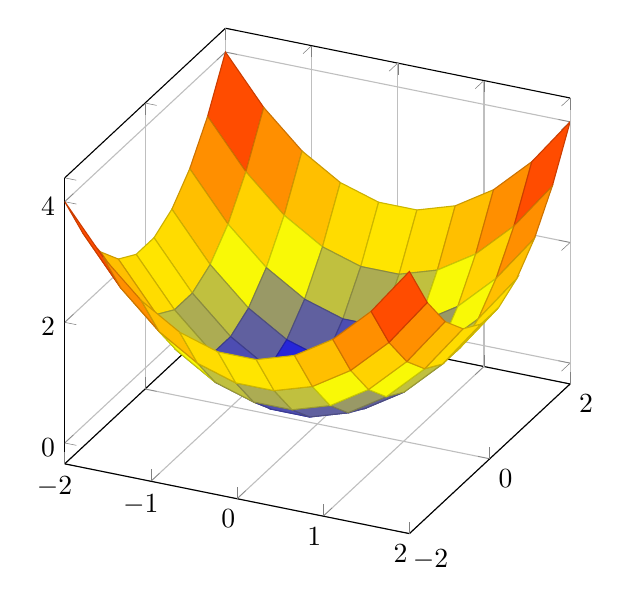
\begin{tikzpicture}
		\begin{axis}[
			domain = -2:2,
			samples = 10,
			y domain = -2:2,
			samples y = 10,
			grid,
			%xtick = { 2 * floor( -2 / 2 ) + 1, 2 * floor( -2 / 2 ) + 3, ...,  2 * floor( 2 / 2 ) + 1 },
			%ytick = { 2 * floor( 0 / 2 ) + 1, 2 * floor( 0 / 2 ) + 3, ...,  2 * floor( 2 / 2 ) + 1 },
			%extra x ticks = { -2, -2 + 1, ..., 2 },
			%extra y ticks = { 0, 0 + 1, ..., 2 },
			%extra x labels = {},
			%extra y labels = {},
			height = 8cm,
			width = 8cm,
		]
			\addplot3[surf] {1/2 * (x^2 + y^2)};
		\end{axis}
	\end{tikzpicture}
	\[
		Df(x_1, x_2) = (x_1, x_2)
	\]
	\[
		Df(1, 1) = (1, 1)
	\]
\end{example}

\begin{example}
	\[
		g : (x_1, x_2) \mapsto \exp \left( -\frac{ 1 }{ 2 } \left( x_1^2 + x_2^2 \right)  \right) 
	\]
	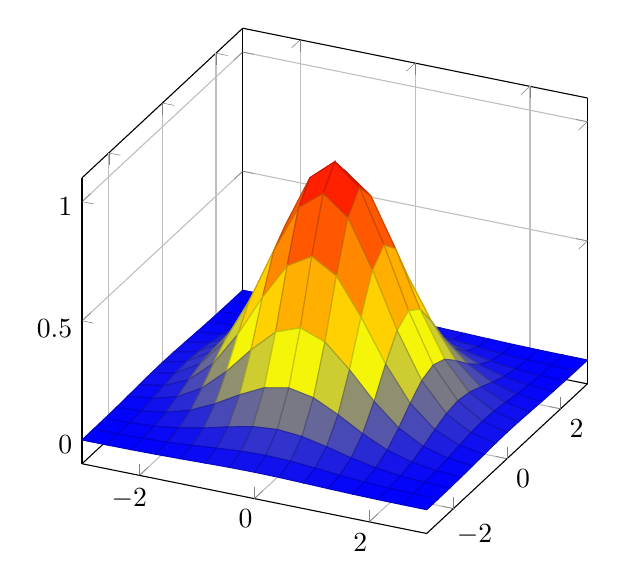
\begin{tikzpicture}
		\begin{axis}[
			domain = -3:3,
			samples = 15,
			y domain = -3:3,
			samples y = 15,
			grid,
			%xtick = { 2 * floor( -2 / 2 ) + 1, 2 * floor( -2 / 2 ) + 3, ...,  2 * floor( 2 / 2 ) + 1 },
			%ytick = { 2 * floor( 0 / 2 ) + 1, 2 * floor( 0 / 2 ) + 3, ...,  2 * floor( 2 / 2 ) + 1 },
			%extra x ticks = { -2, -2 + 1, ..., 2 },
			%extra y ticks = { 0, 0 + 1, ..., 2 },
			%extra x labels = {},
			%extra y labels = {},
			height = 8cm,
			width = 8cm,
		]
			\addplot3[surf] {exp(-1/2 * (x^2 + y^2))};
		\end{axis}
	\end{tikzpicture}
	\[
		Dg(x_1, x_2) = (-x_1, -x_2) \exp \left( -\frac{ 1 }{ 2 } \left( x_1^2 + x_2^2 \right)  \right) 
	\]
	\[
		Dg(1, 1) = (-1, -1) \frac{ 1 }{ e } 
	\]
	
\end{example}

\begin{theorem}
	Sei $ \Omega \subset \R ^n $ offen $ f : \Omega \to \R  $ stetig differenzierbar.
	Wir nennen dann $ \mathcal{N} _f (c) \coloneqq \left\{ x \in \Omega : f(x) = c \right\}  $, $ c \in \R  $ die \textbf{Niveaumenge} von $ f $ zum Wert $ c $.

	Dann steht $ Df(x) $ für $ x \in \mathcal{N} _f(c) $ senkrecht in folgendem Sinne:\\
	Ist $ \varphi : (- \varepsilon , \varepsilon ) \to \R ^n $ mit $ \varphi\left( \left( - \varepsilon , \varepsilon  \right)  \right) \subset \mathcal{N} _f (c) $ mit $ \varphi(0) = x $ stetig differenzierbar, so $ \left< \varphi^\prime (0), Df(x) \right> = 0 $ 
\end{theorem}
\begin{proof*}[Theorem \ref{4.29}]
	Definiere
	\[
		g(t) \coloneqq f\left( \varphi(t) \right) = c
	\]
	dann
	\[
		\underbrace{(Df) (\varphi(t))}_{Df(0)} \underbrace{D\varphi(t)}_{\varphi^\prime (0)} = 0
	\]
	
\end{proof*}

\begin{theorem*}
	Sei $ \Omega \subset \R ^n $, $ x_0 \in \Omega $, $ f : \Omega \to \R ^m $.
	Sei $ \xi \in \R ^n $ so, dass
	\[
		[x_0, x_0 + \xi] \coloneqq \left\{ x_0 + t \xi : 0 \leq t \leq 1 \right\} \subset \Omega.
	\]
	Ist $ f $ stetig differenzierbar, so
	\[
		f\left( x_0 + \xi \right) - f(x_0) = \int_{0}^{1} \underbrace{Df}_{\in \R ^{m \times n} } (x_0 + t \xi ) \dd t \cdot \xi.
	\]
	Hierbei setzen wir für
	\[
		A : [y, b] \to \R ^{m \times n} ,
	\]
	wobei $ A(x) = \left( a_{ij} (x) \right) _{i = 1, \dotsc, m, j = 1, \dotsc, n}  $:
	\[
		\int_{a}^{b} A(x) \dd x \coloneqq \left( \int_{a}^{b} a_{ij} (x) \dd x \right) _{ij} .
	\]
\end{theorem*}
\begin{proof*}[Thm. 2.29]
	$ g(t) \coloneqq  f(x_0, + t\xi) $. Dann
	\begin{align*}
		f(x_0 + \xi) - f(x_0) &= g(1) - g(0) \\
				      &= \begin{pmatrix} g_1(1) - g_1(0) \\ \vdots \\ g_m (1) - g_m(0) \end{pmatrix} \\
				      &= \left( g_k(1) - g_k(0) \right) _{k = 1, \dotsc, m} \\
				      &\overset{\text{Hauptsatz} }{=} \left( \int_{0}^{1} \frac{ \dd }{ \dd t } g_k (t) \dd t \right) _{k = 1, \dotsc, m}  \\
				      &= \left( \int_{0}^{1} \frac{ \dd }{ \dd t } f_k (x_0 + t \xi) \right)_{k = 1, \dotsc, m}   \\
				      &\overset{\text{Kettenregel} }{=} \left( \left< \int_{0}^{1} \mathbf{Df_k} (x_0 + \xi) \dd t, \xi \right> \right) _{k = 1, \dotsc, m}  \\
				      &= \int_{0}^{1} \underbrace{Df}_{\R ^{m \times n} } (x_0 + t \xi) \dd t \cdot \underbrace{\xi}_{\R ^{n \times 1} } \qed
	\end{align*}
\end{proof*}

\begin{theorem}[Schraukensatz]
	In der Situation von Thm 4.29 gilt
	\[
		\left\| f(x_0 + \xi) - f(x_0) \right\| _2 \leq M \left\| \xi \right\| _2, 
	\]
	wobei
	\[
		M \coloneqq  \sup_{0 \leq t \leq 1}  \left\| \left( Df \right) \left( x_0 + t \xi \right)  \right\| 
	\]
	Operatornorm, Lemma \ref{4.22}
\end{theorem}
\begin{proof*}[Thm \ref{4.30}]
	Nach Thm. 4.29:
	\begin{align*}
		\left\| f(x_0 + \xi) - f(x_0) \right\| _2 &= \left\| \int_{0}^{1} \left( Df \right) \left( x_0 + t\xi \right) \dd t \cdot \xi \right\| _2 \\
		~ \overset{(*)}{\leq } \int_{0}^{1} \left\| Df (x_0 + t\xi) \cdot \xi \right\| _2 \dd t \\
		~ & \leq \int_{0}^{1} \underbrace{\left| (Df) (x_0 + t\xi) \right| }_{\leq M} \cdot \left| \xi \right| _2 \dd t \\
		~ & \leq M \cdot \left\| \xi \right\| _2.
	\end{align*}
	\textbf{Zu $ (*) $}: Ist $ v : [a, b] \to \R ^m $ stetig.
	Dann:
	\[
		\left\| \int_{a}^{b} v(t) \dd t \right\| _{2} \leq \int_{a}^{b} \left\| v(t) \right\| _2 \dd t.
	\]
	Sei hierzu
	\[
		\eta \coloneqq \int_{a}^{b} v(t) \dd t = \begin{pmatrix} \int_{a}^{b} v_1(t) \dd t \\ \vdots \\ \int_{a}^{b} v_m (t) \dd t \end{pmatrix} 
	\]
	Definiere
	\begin{align*}
		K \coloneqq \left\| \eta \right\| _2 \implies K^2 &= \left\| \eta \right\| _2^2 \\
		~ &= \left< \eta, \eta \right> \\
		~ &= \left< \int_{a}^{b} v(t) \dd t, \eta \right> \\
		  &= \int_{a}^{b} \left< v(t \right> \\
		  & \overset{\text{Cauchy-Schwarz} }{\leq } \int_{a}^{b} \left\| v(t) \right\| _2 \cdot \underbrace{\left\| \eta \right\| _2}_{K} \dd t \\
		  &= K \int_{a}^{b}\left\| v(t) \right\| _2 \dd t.
	\end{align*}
	\OE{} $ K \neq 0 $, kürze durch $ K $.\qed
\end{proof*}

